\chapter{\MIndex{}}

V~této části je popsán a vybudován Metrický Index --- jeho principy, architektura a prohledávání.
Text a obrázky v~této kapitole jsou vlastním volným překladem nebo převzaty s~odpovídajícím označením z~původního popisu \MIndex{u}\cite{Novak:2009:MIE:1637863.1638184}.

\section{\MIndex{} prvního stupně}

Jak bylo již zmíněno, koncept \MIndex{u} je inspirován iDistance, která je indexovací metodou pro podobnostní vyhledávání ve vektorovém prostoru.
Pokud máme vzorovou množinu $S\subseteq\mathbb{\mathcal{D}}$, pak iDistance rozdělí $S$ na $n$~clusterů a utvoří referenční bod $p_{i}$ pro každý cluster $C_{i},\: i\in\left\{ 0,\ldots,n-1\right\} $.
Každému prvku $o\in X$ je pak přiřazen číselný klíč odpovídající vzdálenosti od referenčního prvku clusteru.
Pokud máme dostatečně velkou konstantu $c$ pro oddělení jednotlivých clusterů, pak iDistance klíč pro prvek
$o\in C_{i}$ je
\[
iDist(o)=d(p_{i},o)+i\cdot c
\]


Tento vzorec mapuje všechny prvky z~jakéhokoliv clusteru $C_{i}$ do intervalu $[i\cdot c,(i+1)\cdot c]$ --- viz \ref{fig:iDistance}.
Datové objekty jsou poté uloženy do \BPTree{} podle jejich \emph{iDist} klíčů.
Při prohledávání je iDistance prostor procházen podle principu -- pro \emph{range query} $R(q,r)$ můžeme určit několik intervalů
\emph{iDist} klíčů, které musejí být vyhodnoceny v~rámci dotazu.

\begin{figure}[t]
\center
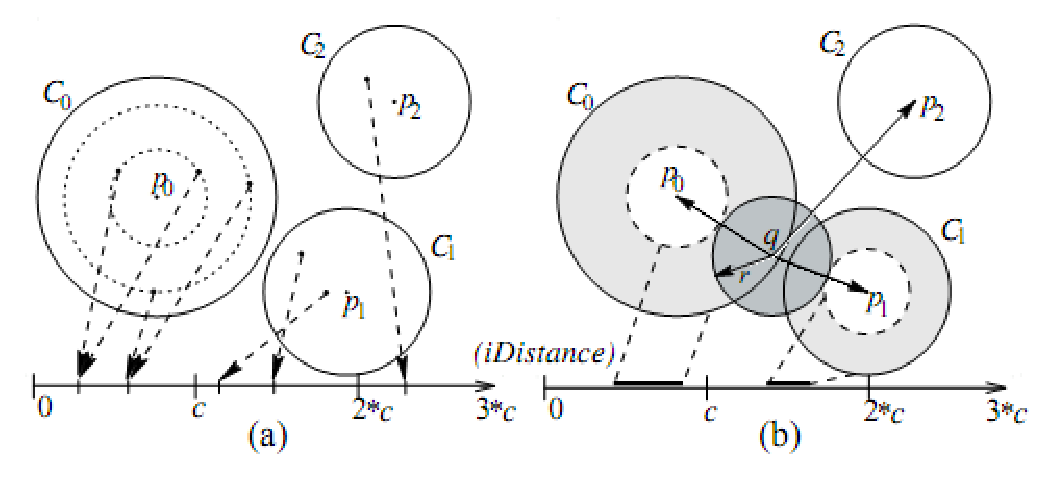
\includegraphics[clip,scale=0.4]{idistance}

\caption{iDistance}
\label{fig:iDistance}
\end{figure}

\MIndex{} zobecňuje iDistance tak, že může být použit na~obecné metrické prostory -- ne jenom na vektorový prostor.
Toho je dosaženo tím, že se vybere množina $n$~pivotů $p_{0},p_{1},\ldots,p_{n-1}$ a apriori ze vzorové množiny $S\subseteq\mathcal{D}$ a poté aplikováním Voroného dělení a rozdělení prostoru na $n$~clusterů. \prettyref{fig:M-Index-level-one} ukazuje příklad takového rozdělení ve 2D pro 4 pivoty ($n=4)$.

\begin{figure}[t]
\center
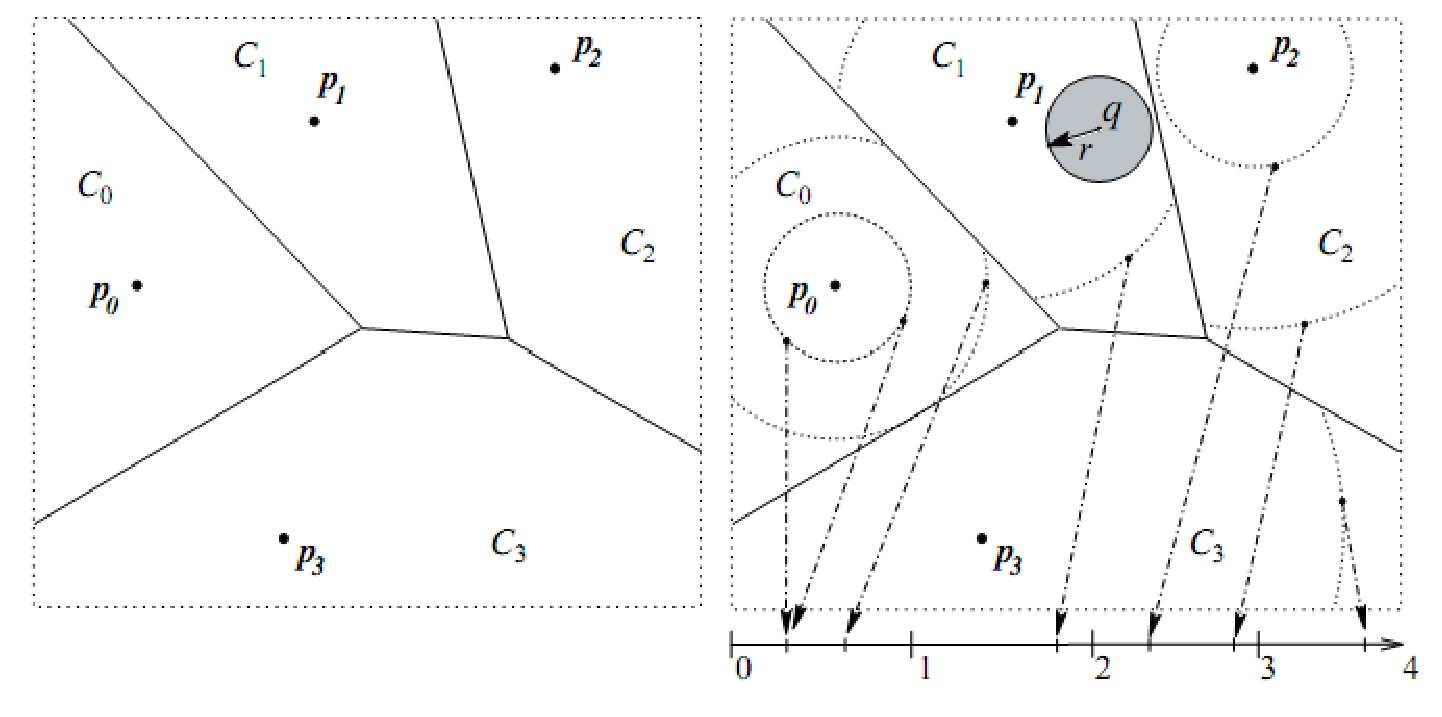
\includegraphics[scale=0.5]{m-index-level-one}
\caption{\MIndex{} prvního stupně $(l=1)$}
\label{fig:M-Index-level-one}
\end{figure}

\section{Vícestupňový \MIndex{}}

Aby byl \MIndex{} škálovatelný pro~rostoucí množství dat, budeme chtít
aplikovat další rozdělování clusterů. Pro~daný cluster $n$~pivotů
$\{p_{0},p_{1},\ldots,p_{n-1}\}$ a prvek $o\in\mathcal{D}$, platí

\[
(\cdot)_{o}\,:\,\{0,1,\ldots,n-1\}\rightarrow\{0,1,\ldots,n-1\}
\]

je permutace indexů tak, že

\[
d(p_{(0)_{o}},o)\leq d(p_{(1)_{o}},o)\leq\cdots\leq d(p_{(n-1)_{o}},o)
\]
Jinak: řada $p_{(0)_{o}},p_{(1)_{o}},\ldots,p_{(n-1)_{o}}$ je seřazena
podle vzdáleností mezi pivoty a prvkem $o$\@.

\MIndex{} s~$l$ stupni, kde $l$ je celé číslo $1\leq l\leq n$, rozděluje
prostor $\mathcal{D}$ do $n\cdot(n-1)\cdot\cdots\cdot(n-l+1)$ clusterů
za použití rekursivního Voroného dělení: Na prvním stupni je každý
prvek $o\in\mathcal{D}$ přiřazen k~jeho nejbližšímu pivotu $p_{(0)_{o}}$ --
takto se utvoří clustery $C_{i}$\@.
Na druhém stupni se každý cluster
$C_{i}$ rozdělí na $n-1$ clusterů tím samým způsobem s~použitím
$n-1$ pivotů $\{p_{1},\ldots,p_{i-1},p_{i+1},\ldots,p_{n}\}$ a vytvořením
clusterů $C_{i,j}$\@. Jinými slovy, cluster $C_{i,j}$ je tvořen
prvky $o\in X$, pro které pivot $p_{i}$ je nejbližší a $p_{j}$
je druhý nejbližší: $(0)_{o}=i$ a $(1)_{o}=j$\@.
Tento postup je zopakován $l$-krát\@.

\begin{figure}[t]
\centering{}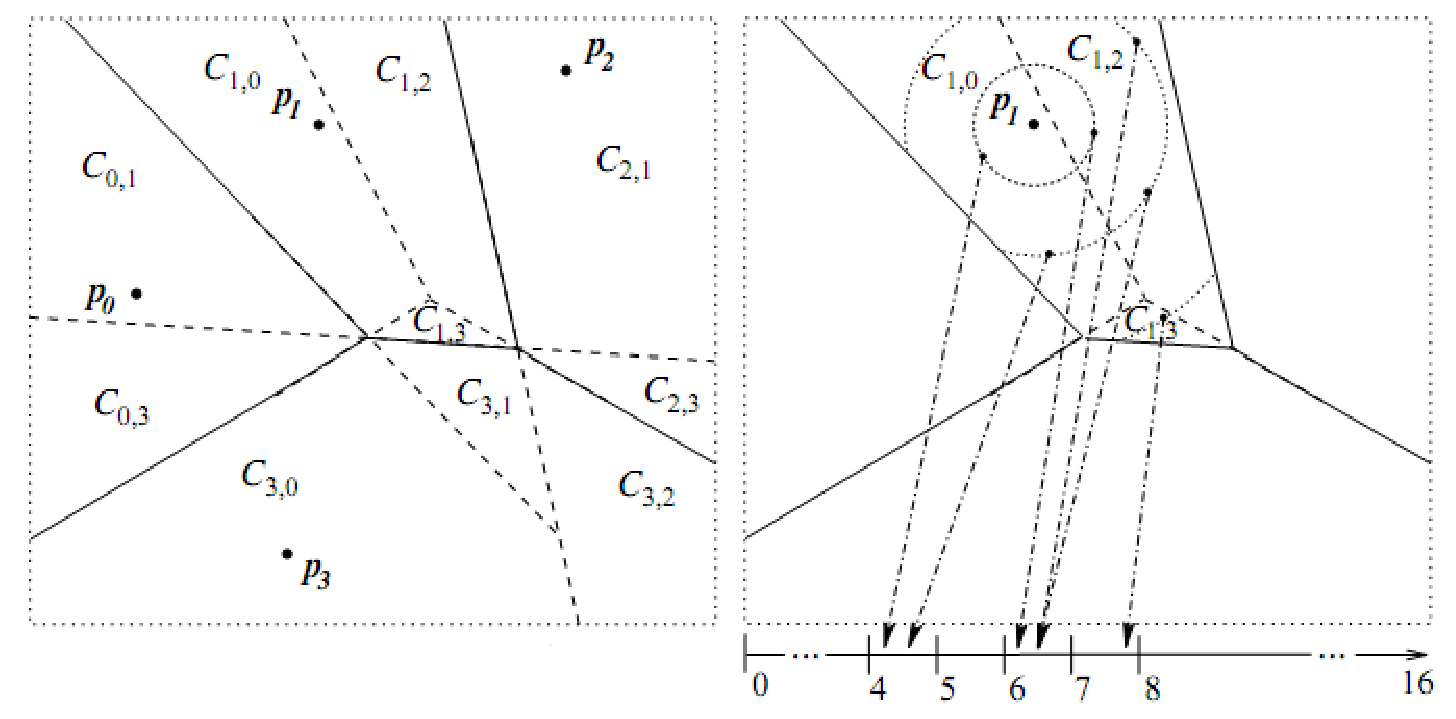
\includegraphics[scale=0.5]{m-index-level-two}\caption{\MIndex{} druhého stupně $(l=2)$}
\label{fig:M-Index-level-two}
\end{figure}


Mapovací klíč \MIndex{u} je definován $key_{l}\,:\,\mathcal{D\rightarrow\mathbb{R}}$\@.
Nechť $o\in\mathcal{D}$ patří do clusteru $C_{i_{0},i_{1},\ldots,i_{l-1}}$\@.
Celočíselná část klíče $key_{l}(o)$ identifikuje cluster: je rovna
číslu \uv{$i_{0}i_{1}\ldots i_{l-1}$'}. Desetinná část klíče $key_{l}(o)$
je vzdálenost mezi prvkem $o$ a jeho nejbližším pivotem $d(p_{(0)_{o}},o)$\@.
Celé mapování \MIndex{u} vyjádříme následujícím vztahem\cite{Novak:2009:MIE:1637863.1638184}

\begin{equation}
key_{l}=d(p_{(0)_{o}},o)+\sum_{i\text{=0}}^{l-1}(i)_{o}\cdot n{}^{(l-1-i)}\label{eq:M-Index-key}
\end{equation}


\prettyref{fig:M-Index-level-two}\cite{Novak:2009:MIE:1637863.1638184} zobrazuje mapování pro dvoustupňový
\MIndex{} $(l=2)$\@. Velikost domény je $4^{2}=16$ a prvky z~clusteru
$C_{i,j}$ jsou mapovány do intervalu $[i\cdot n+j,i\cdot n+j+1]$\@.


\section{\MIndex{} s~dynamickými stupni\label{sec:Dynamic-Cluster-Tree}}

Vícestupňový \MIndex{} zlepšuje dělící schopnosti oproti jednostupňovému \MIndex{u} seskupováním/shromažďováním blízkých prvků do menších clusterů\@.
Teoreticky, čím více stupňů \MIndex{} má, tím je vyhledávání efektivnější.
Na druhou stranu, velké množství malých clusterů vede k~větší fragmentaci dat při dotazu a větší náročnosti při provádění dotazu.
V~praxi to vede ke ztrátě výhody z~vícestupňovosti.

Koncept \MIndex{u} může být rozšířen o~dynamický počet stupňů, který umožní \prettyref{eq:M-Index-key} dynamicky zvětšovat (prohlubovat) pro velké clustery, protože \prettyref{eq:M-Index-key-max-level} požaduje pouze lokální změny klíčů \MIndex{u}
Toto vylepšení vyžaduje následující modifikace:
\begin{itemize}
\item je vybrán fixní \uv{maximální stupeň \MIndex{u}} $1\leq l_{max}\leq n$
a doména pro~tento maximální stupeň $n^{l_{max}}$ je alokována
\item rovnice \prettyref{eq:M-Index-key} pro $key_{l}$ stupně $l,\,1\leq l\leq l_{max}$
je změněna na\cite{Novak:2009:MIE:1637863.1638184}:
\begin{equation}
key_{l}=d(p_{(0)_{o}},o)+\sum_{i\text{=0}}^{l-1}(i)_{o}\cdot n{}^{(l_{max}-1-i)}\label{eq:M-Index-key-max-level}
\end{equation}

\item je vytvořen dynamický \emph{cluster tree}, který určuje aktuální hloubku
pro dané \MIndex{} clustery
\end{itemize}
Jak vypadá taková stromová struktura pro $l_{max}=3$ je zobrazeno
na~\prettyref{fig:Dynamic-Cluster-Tree}\cite{Novak:2009:MIE:1637863.1638184}. Prvky mají přiřazeny
klíče v~nejnižších patrech (listech). Typicky se nastaví limit na
možný počet prvků/dat uložených v~clusteru a zvýší se stupeň clusteru
při jeho zaplnění.

\begin{figure}[t]
\centering
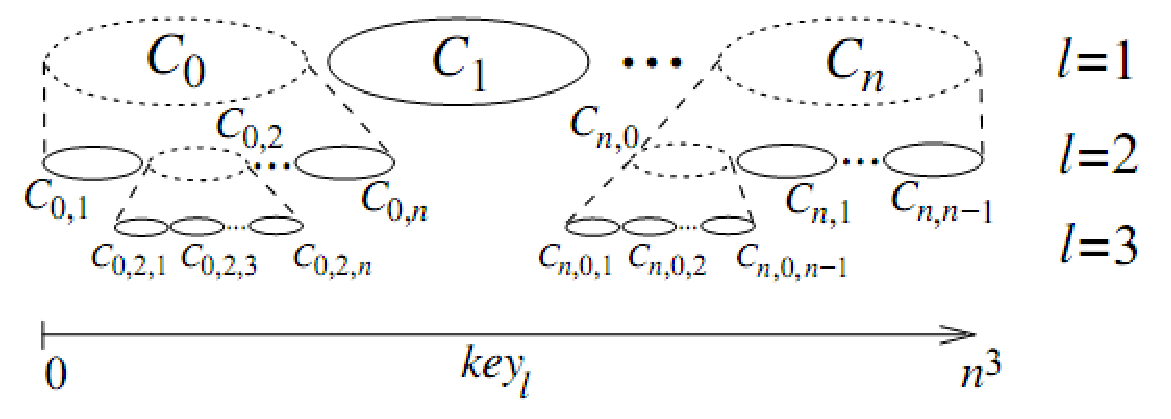
\includegraphics[scale=0.5]{m-index-dynamic-cluster}
\caption{Dynamický \MIndex{}}
\label{fig:Dynamic-Cluster-Tree}
\end{figure}

Rozdělení clusteru o~jeden stupeň znamená lokální přetřídění prvků
patřících do clusteru. Pokud zarovnáme počet pivotů~$n$ na násobky
2, pak každý stupeň $key_{l},\,1\leq l\leq l_{max}$ definuje určitý
počet bitů integrální části $key_{l_{max}}$\@. Toto přiřazení je
velmi podobné \emph{extensible hashing}\cite{Fagin:1979:EHF:320083.320092}
a rozdělení takového clusteru znamená zohlednění dalších bitů z~$key_{l_{max}}$\@.
V~praxi je $l_{max}$ limitován pouze $n$, případně rozsahem číselné
reprezentace $key$ \@.


\section{Range Query\label{sec:Range-Query}}

Zde popíšeme algoritmus \emph{range~query} $R(q,r)$ jako základní
dotaz podobnosti.

V~prvním kroku se spočítají vzdálenosti $d(p_{i},q),\, i=1,\ldots,n$,
všech $n$~pivotů k~dotazovanému prvku (objektu)\@. Algoritmus
bere v~potaz všechny clustery na stupních $1,\ldots,l$ (pro fixní
\MIndex{} nebo projde celý strom clusterů (\emph{cluster~tree})\@.
Díky opakovanému Voroného dělení a podle \emph{Double-Pivot Distance
Constraint}\cite{similaritysearch2006}, cluster $C_{i}$ může být
vynechán, pokud
\[
d(p_{i},q)-d(p_{(0)_{q}},q)>2\cdot r
\]
kde $p_{(0)_{q}}$ je pivot nejbližší ke~$q$\@. Protože Voroného
dělení je opakováno $l$-krát pro stupeň $l$, toto pravidlo může
být opakováno $l$-krát pro cluster $C_{i_{0},\ldots,i_{l-1}}$\@.
Na každém stupni $j,\,1\leq l\leq l$ jsou pivoty $p_{i_{0},\ldots,i_{j-2}}$
ignorovány omezovacím mechanismem, protože byly vynechány Voronovým
dělením na stupni $l$\@.

Znalostí minimální a maximální vzdáleností mezi pivoty v~clusteru
(který jsou uloženy v~listech stromu), můžeme uplatnit \emph{Range Pivot
Distance Constraint}\cite{similaritysearch2006} a nemusíme přistupovat
ke clusteru $C_{p,*}$ pokud
\[
d(p,q)+r<r_{min} \wedge d(p,q)-r>r_{max}
\]
kde $r_{min}$ a $r_{max}$ je minimální a maximální vzdálenost prvků
v~daném clusteru\@.

Pokud žádný z~výše uvedených filtrujících mechanismů neodfiltruje
cluster $C_{i_{0},\ldots,i_{l-1}}$ na úrovni listů, pak můžeme určit
interval pro $key$ domény, které mají být prohledány v~tomto clusteru:
\[
[d(p_{i_{0},}q)-r,d(p_{i_{0}},q)+r]
\]

kde oba limity jsou posunuty o~celočíselnou část klíčů clusteru $C_{i_{0},\ldots,i_{l-1}}$ podle
$key_{l}$ rovnic \prettyref{eq:M-Index-key} nebo \prettyref{eq:M-Index-key-max-level}.
Tento mechanismus je \uv{vypůjčen} \linebreak z~iDistance a je přímou aplikací
\emph{Object-Pivot Distance Constraint}\cite{similaritysearch2006}.

\section{Architektura \MIndex{u}}

V~předchozích sekcích byly uvedeny algoritmy a mechanismy, které
nutí k~použití různých specifických datových struktur\@. Obecně,
datové prvky mohou být uloženy v~jakékoliv struktuře, která je indexuje
podle jejich \MIndex{} klíčů. Ideální je efektivní vyhodnocování přes
intervalové dotazy -- \BPTree{}\cite{Cormen:2001:IA:580470}%
\footnote{detailní popis \BPTree{} viz \prettyref{sub:B-plus-tree}%
} je typickým představitelem takovéto struktury\@.

Implementace stromu clusterů (\emph{cluster tree}) je jednoduchá\@.
Záznam pro cluster $C_{i_{0},\ldots,i_{l-1}}$ je z: $l$, pole $\left\langle i_{0},\ldots,i_{l-1}\right\rangle $
a buď ukazatelů na podstromy $\left\langle sub_{0},\ldots,sub_{n-1}\right\rangle $
v~případě vnitřního uzlu nebo $r_{min},\, r_{max}$ pro záznam listu\@.
Strom clusterů by měl být udržován v~hlavní paměti.
